\documentclass[letterpaper]{article}
\usepackage[submission]{aaai2027}
\usepackage[hyphens]{url}
\usepackage{graphicx}
\urlstyle{rm}
\def\UrlFont{\rm}
\usepackage{natbib}
\usepackage{caption}
\frenchspacing
\usepackage{booktabs}

\pdfinfo{
/TemplateVersion (2027.1)
}

\title{Equal-Budget Observation-Condition Randomization Improves Synthetic Einstein-Radius Regression Robustness}
\author{Anonymous Submission}
\affiliations{}

\begin{document}
\maketitle

\begin{abstract}
Observation mismatch can degrade learned strong-lens parameter estimates, but extra augmented images and optimizer updates can confound the apparent benefit of randomization. We evaluate a convolutional regressor for the angular Einstein radius under a matched training budget. Canonical training (C), uniform observation-condition variation (G), and a source-development failure-weighted policy (R) use the same architecture, initialization, source-parent schedule, 880 updates, batch size, and source-image exposure. On a frozen parent-disjoint synthetic holdout, four-stress mean absolute error (MAE) was 0.141251 arcsec for C and 0.111507 arcsec for G. The paired change G--C was -0.029744 arcsec (parent-bootstrap 95\% interval [-0.045725,-0.012141]). R obtained 0.107385 arcsec, but R--G was inconclusive. A separate AutoLens/Lenstronomy audit produced byte-identical saved image pairs. We therefore claim bounded synthetic robustness, not simulator transfer, real-observation accuracy, or superiority over published methods.
\end{abstract}

\section{Introduction}

Artificial intelligence is increasingly used as a scientific instrument: it
can replace expensive inference steps, expose sensitivity to experimental
conditions, and support decisions about where computational effort is most
useful. Strong gravitational lensing is a compact test case for this problem.
Convolutional models can estimate lens parameters quickly, but their errors can
change when pixel scale, exposure, detector noise, or rendering conventions
change. A result that improves only because it receives more updates or more
images is difficult to interpret as a robustness intervention.

We ask a deliberately narrow question: when architecture, optimizer, update
count, initialization, source-parent schedule, and source-image exposure are
matched, does source-only variation of observation conditions improve
Einstein-radius prediction on unseen synthetic lens systems? The study is a
reliability measurement rather than a new CNN architecture. It separates the
effect of condition exposure from additional optimization, reports a negative
result for a failure-weighted allocation policy, and audits a proposed
alternate renderer rather than assuming that a package change creates a domain
shift.

Our central result is a paired four-stress MAE reduction for uniform variation
relative to canonical training under an equal budget. The claim is bounded to
the declared synthetic generator, prior, preprocessing and stress conditions.
We do not compare our MAE numerically with incompatible published $R^2$,
signed-residual, uncertainty-coverage, or real-data results.

\section{Related Work}

CNN inference of strong-lens parameters is established by
\citet{hezaveh2017fast}; observational variation and simulation diversity have
also been studied for lens-light, signal-to-noise, and mass/light effects
\citep{pearson2019effect}. The closest domain-shift studies use domain
adaptation for Einstein-radius inference. Swierc et al. compare DANN and MMD
between simulated source and DES-like target domains
\citep{swierc2023domain}, while Agarwal et al. combine MMD with mean-variance
prediction and uncertainty evaluation \citep{agarwal2024domain}. These methods
use unlabeled target images during adaptation and report objectives that are
not identical to our source-only point-MAE setting.

Gawade et al. study increasing simulation realism and HSC-oriented real-image
comparisons \citep{gawade2025cnn}; their real-data evidence is outside the
scope of our synthetic benchmark. Galan et al. demonstrate that explicit
convention handling is central to cross-code lens modeling
\citep{galan2024comparison}. More general domain-randomization and augmentation
methods, including active domain randomization and RandAugment, establish that
preferential or randomized variation is not itself a new algorithmic idea
\citep{mehta2020active,cubuk2020randaugment}.

The contribution here is therefore a controlled attribution result: a
parent-safe, target-free comparison of condition exposure under matched
training effort, together with an explicit boundary on what an alternate
renderer audit can establish.

\section{Task and Data}

Each synthetic image contains an SIE lens, extended S\'ersic source and lens
light, an unresolved lensed point source, a Gaussian point-spread function
(PSF), and a simplified detector/noise model. The target is the simulator's
angular Einstein radius $\theta_E$ in arcseconds. The CNN receives image pixels
and returns one scalar. Source training uses 697 qualified parents; the frozen
holdout contains 150 parents and was not used for fit selection. Parent IDs,
not rendered views, define statistical independence.

The primary holdout includes a canonical condition and four predefined stresses:
native pixel scale 0.04 and 0.06 arcsec/pixel, half exposure, and doubled read
noise. The four-stress endpoint is the equal-weight MAE averaged across the
four stress views within each parent. Canonical MAE is a guardrail and is not
included in the stress composite.

\section{Matched-Budget Study}

\subsection{Training arms}

All arms use the same CNN, AdamW optimizer, Huber loss, normalization policy,
initial weights, batch size 16, and 880 optimizer updates per seed. Ten paired
seeds (730001--730010) are fit for each arm. Within each seed, the arms share
the same realized source-parent schedule and expose the same number of source
images.

\begin{itemize}
\item \textbf{C}: canonical observation only.
\item \textbf{G}: uniform sampling over the frozen observation-condition cells.
\item \textbf{R}: source-development failure-weighted sampling over the same cells.
\end{itemize}

The failure-weighted policy is fixed before final fitting from source-
development errors. No holdout images or labels are used to choose policies,
checkpoints, or normalization. Fits and predictions are target-free; the
holdout target join occurs only after predictions are sealed.

\subsection{Metrics and uncertainty}

The primary contrast is G--C in parent-averaged four-stress MAE. Secondary
contrasts are R--G and R--C. Percentile intervals use 10,000 bootstrap
resamples of the 150 independent parents, keeping condition views grouped
within each parent. Training-seed variation is reported separately rather than
treated as additional astronomical systems.

\section{Results}

\subsection{Equal-budget performance}

\begin{table}[t]
\centering
\caption{Equal-budget performance on the frozen synthetic holdout.}
\label{tab:main}
\begin{tabular}{lcc}
\toprule
Arm & Canonical MAE & Four-stress MAE \\
 & (arcsec) & (arcsec) \\
\midrule
C: canonical & 0.091536 & 0.141251 \\
G: uniform variation & 0.087591 & 0.111507 \\
R: failure-weighted & 0.092366 & 0.107385 \\
\bottomrule
\end{tabular}
\end{table}

Uniform variation reduced four-stress MAE relative to canonical training by
$-0.029744$ arcsec, with a parent-bootstrap 95\% interval
$[-0.045725,-0.012141]$. This interval excludes zero and supports an
equal-budget robustness effect for the tested synthetic stresses. The
failure-weighted policy obtained lower point MAE than G, but its R--G contrast
was $-0.004122$ arcsec with interval $[-0.026208,0.009341]$; the study does
not establish an additional benefit from weighting.

\begin{figure}[t]
\centering
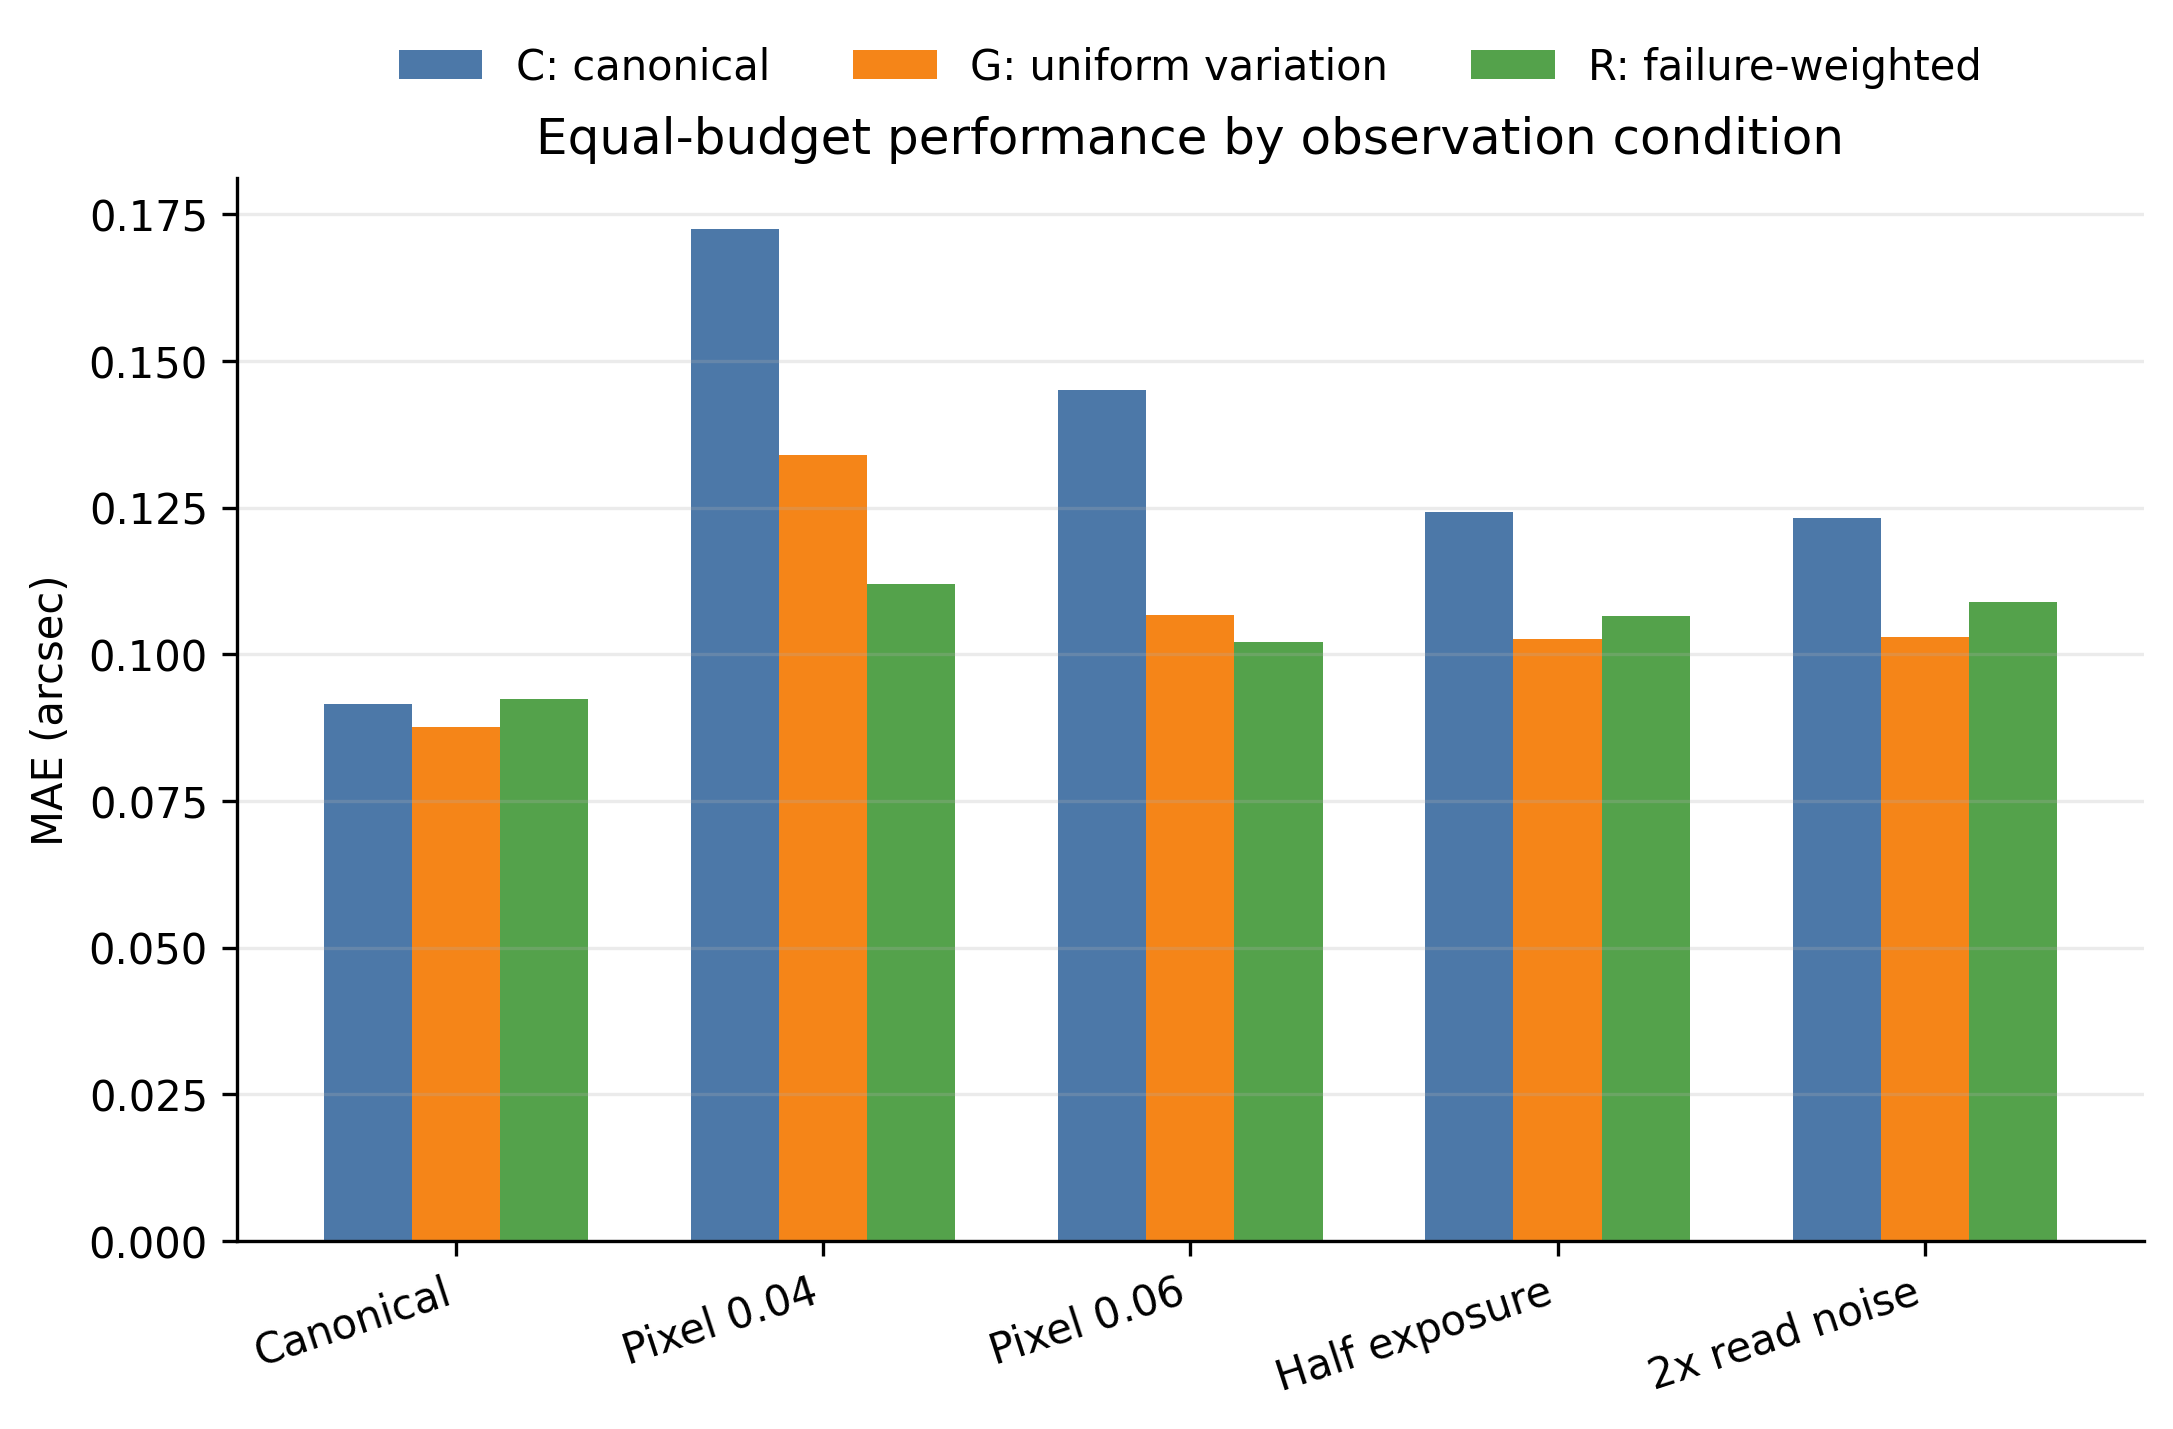
\includegraphics[width=\columnwidth]{figures/equal_budget_mae_by_condition.png}
\caption{MAE by observation condition for the three equal-budget arms.}
\label{fig:mae}
\end{figure}

\begin{figure}[t]
\centering
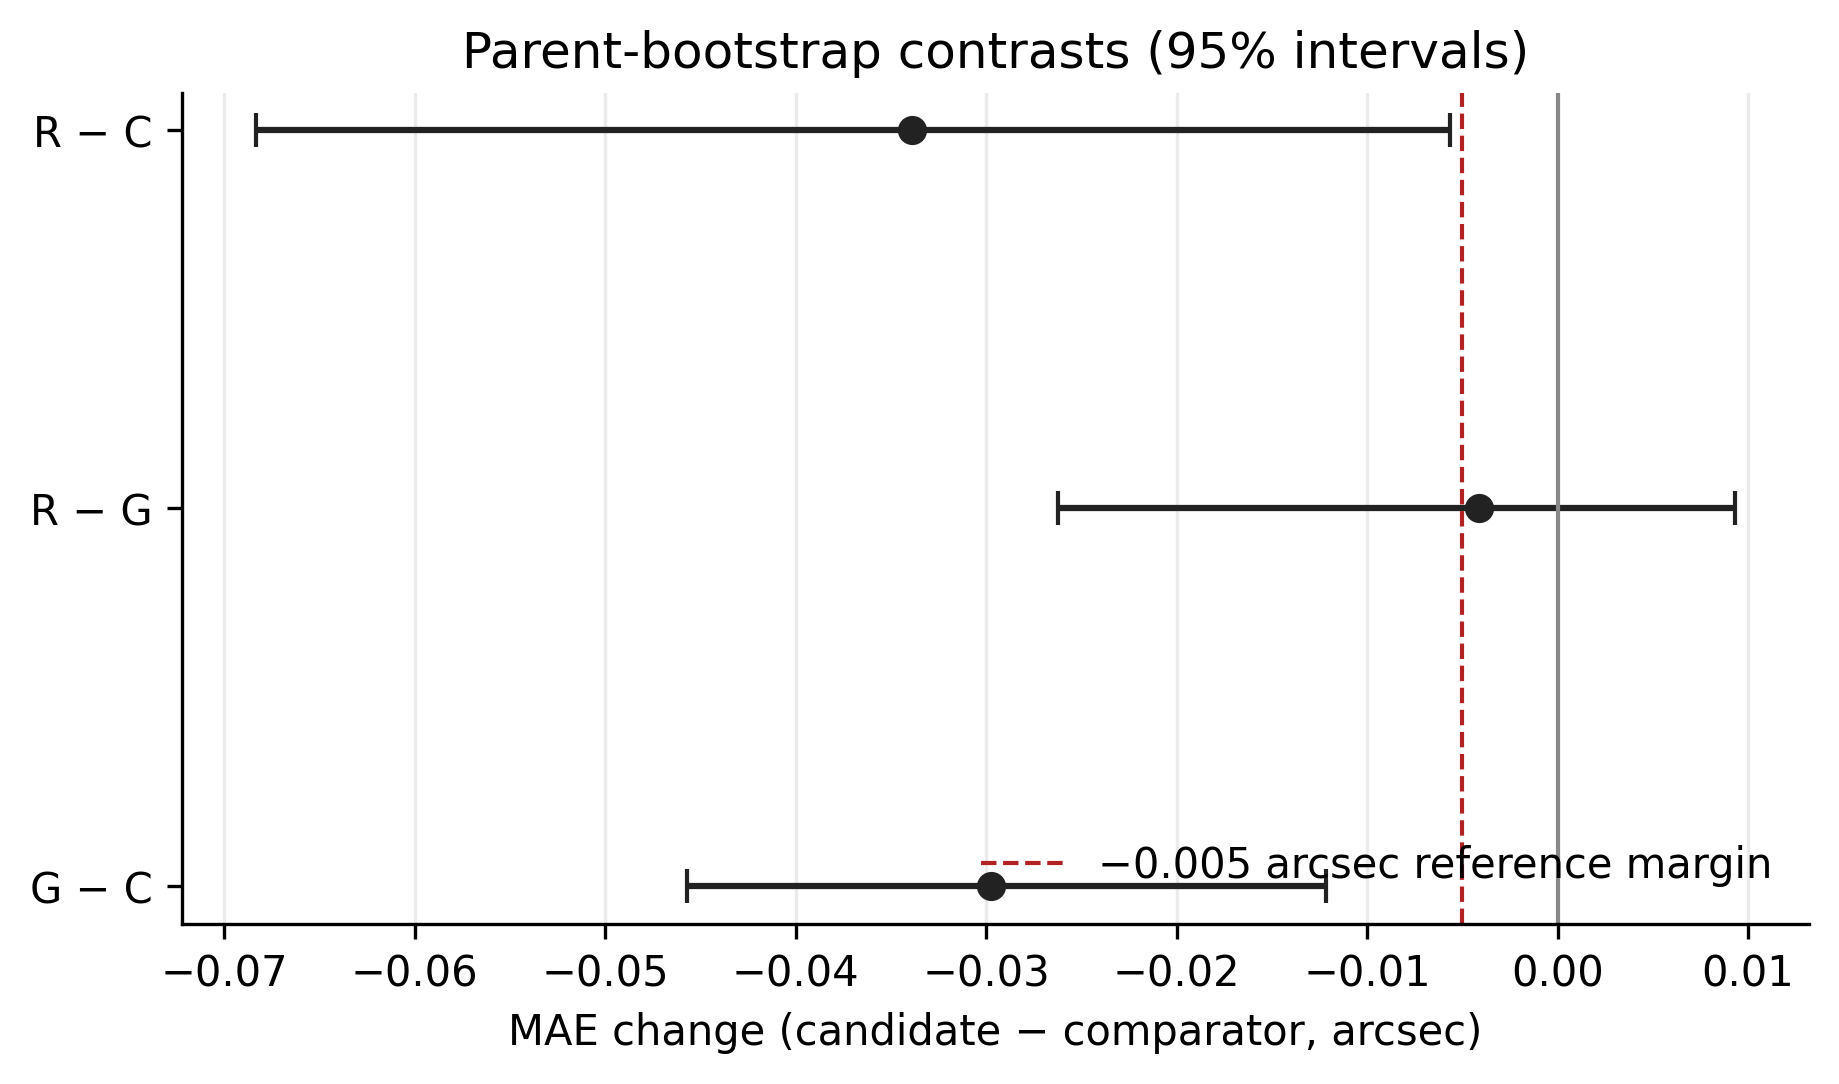
\includegraphics[width=\columnwidth]{figures/equal_budget_paired_contrasts.png}
\caption{Parent-bootstrap paired contrasts. Negative values favor the candidate arm.}
\label{fig:contrasts}
\end{figure}

The older 27.4\% reduction came from a historical canonical-versus-randomized
comparison with unequal update and image-exposure budgets. We retain it as
context, but the equal-budget contrast above is the causal estimate used here.

\subsection{Renderer audit and unseen PSF family}

As a secondary engineering evaluation, fixed checkpoints were applied to 150
new paired parents rendered through the project Lenstronomy and AutoLens paths
under nine conditions, including three Moffat-PSF cells absent from source
training. Predictions were sealed before labels were joined. All 1,350 paired
image products and all 40,500 paired predictions were exactly equal at saved
precision. The Moffat cells therefore measure an unseen observation-family
shift shared by both renderer labels; they do not measure a simulator-induced
image-domain shift.

\section{Discussion and Limitations}

The result is relevant to AI for science because it identifies a practical
failure mode---observation-condition mismatch---and measures a mitigation under
controlled computational effort. It also shows why engineering provenance is
part of the scientific result: a different package version does not establish
a different model input distribution when convention conversion and image
formation are shared.

The benchmark uses one synthetic parent prior, one scalar target, and a
project-specific PSF, detector, and preprocessing stack. The Moffat family is
engineered synthetic data, not a calibrated telescope PSF. The AutoLens and
Lenstronomy paths share enough image-forming code and matched conventions to
produce identical saved products, so independent simulator transfer remains
future work. The equal-budget holdout is parent-disjoint from training but was
previously scored by older models; this is an independent equal-budget refit on
a frozen holdout, not a never-before-opened dataset.

No real-image $\theta_E$ labels were used. No exact reproduction of the Swierc
or Agarwal methods was run, and no numerical superiority claim over those
papers is made. The observed seed and parent intervals condition on the fixed
source sample and policy-construction procedure.

\section{Conclusion}

When CNN architecture, optimizer updates, initialization, parent schedule and
source-image exposure are matched, source-only observation-condition variation
reduces four-stress Einstein-radius MAE on parent-disjoint synthetic systems.
A failure-weighted allocation does not show a reliable additional gain over
uniform variation. The evidence supports a reproducible synthetic robustness
measurement, not simulator-independent inference, real-data accuracy, or a
published-method leaderboard claim.

\section*{Reproducibility}

The equal-budget runner, sealed predictions, final report, renderer identity
audit, figures, and environment/hash checklist are provided with the
submission supplement. The main result is reproduced from the frozen report
without reopening target labels during fitting or prediction.

\bibliographystyle{aaai2027}
\bibliography{paper}

\end{document}
